% Канонический TikZ-рисунок варианта 22. Править только здесь.
\long\def\figStereoV22{%
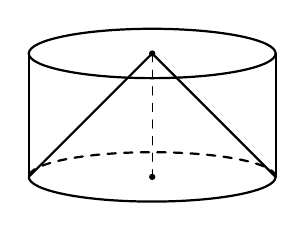
\begin{tikzpicture}[
  scale=0.95,
  line cap=round,
  line join=round
]
  % Высота цилиндра визуально равна радиусу основания
  \def\radius{1.65}
  \def\height{1.65}
  \def\ellipseheight{0.33}

  \coordinate (S) at (0,\height);
  \coordinate (L) at (-\radius,0);
  \coordinate (R) at (\radius,0);
  \coordinate (O) at (0,0);

  % Верхнее основание цилиндра
  \draw[thick]
    (0,\height)
    ellipse[
      x radius=\radius,
      y radius=\ellipseheight
    ];

  % Боковые рёбра цилиндра
  \draw[thick]
    (-\radius,0) -- (-\radius,\height);

  \draw[thick]
    (\radius,0) -- (\radius,\height);

  % Нижнее основание цилиндра
  \draw[thick]
    (L)
    arc[
      start angle=180,
      end angle=360,
      x radius=\radius,
      y radius=\ellipseheight
    ];

  \draw[thick,dashed]
    (R)
    arc[
      start angle=0,
      end angle=180,
      x radius=\radius,
      y radius=\ellipseheight
    ];

  % Конус с теми же основанием и высотой
  \draw[thick]
    (S) -- (L);

  \draw[thick]
    (S) -- (R);

  % Высота конуса
  \draw[dashed]
    (S) -- (O);

  \fill (S) circle (1.2pt);
  \fill (O) circle (1.2pt);
\end{tikzpicture}
}
